\documentclass[a4paper,11pt]{article}

\usepackage[a4paper,top=2cm,bottom=2cm,left=2cm,right=2cm]{geometry}
\usepackage[T1]{fontenc}
\usepackage[utf8]{inputenc}
\usepackage{graphicx}
\usepackage{lmodern}% http://ctan.org/pkg/lm
\usepackage{enumitem}
\usepackage{array}
\usepackage{listings}
\usepackage[italian]{babel}
\usepackage{amsmath}
\usepackage{mathtools}
\usepackage{xspace}
\usepackage{amssymb}


\graphicspath{{./Immagini/}} 

\newcommand{\tab}[1]{\hspace{.3\textwidth}\rlap{#1}}
\newcommand{\itab}[1]{\hspace{0em}\rlap{#1}}
\newcommand{\alc}{%                           ALC
   \ensuremath{\mathcal{ALC}}\xspace}
\newcommand{\I}{%                             I (caligraphic)
        \ensuremath{\mathcal{I}}\xspace}
\newcommand{\Q}{%                             Q
  \ensuremath{\mathcal{Q}}\xspace}
\newcommand{\N}{%                             N
  \ensuremath{\mathcal{N}}\xspace}
\newcommand{\Onom}{%                          O
  \ensuremath{\mathcal{O}}\xspace}
\newcommand{\T}{%                             T
  \ensuremath{\mathcal{T}}\xspace}
\newcommand{\A}{%                             T
  \ensuremath{\mathcal{A}}\xspace}
\newcommand{\K}%                              Modal K
        {\ensuremath{\mathbf{K}}\xspace}

\begin{document}

\begin{figure}[!htbp]
\centering	
	\mbox{%
		\begin{minipage}{.10\textwidth}
			
\includegraphics[scale=0.20]{Immagini/unict.jpg} 
		\end{minipage}%
		\quad
		\begin{minipage}[c]{.60\textwidth}
			\centering
			\Large Universit\`{a} degli Studi di Catania
			
			\Large Dipartimento di Matematica e Informatica
			
			\Large Corso di Laurea in Informatica triennale
			
		\end{minipage}
		}
\end{figure}

\begin{center}
	\hrule
\end{center}

\vspace*{50pt}

\begin{center}
	\LARGE Andrea Costazza
\end{center}

\vspace*{30pt}

\begin{center}
	\LARGE \textbf{Titolo:}

	\LARGE \textbf{sottotitolo}
\end{center}

\vspace*{80pt}

\noindent\hfil\rule{0.2\textwidth}{.4pt}\hfil

\begin{center}
	\Large Relazione progetto finale
\end{center}

\noindent\hfil\rule{0.2\textwidth}{.4pt}\hfil

\vspace*{180pt}

\begin{flushright}
	\Large Relatore

	\Large \textbf {Prof. Domenico Cantone}
\end{flushright}
\begin{flushright}
	\Large Correlatore

	\Large \textbf {Dott. Cristiano Longo}
\end{flushright}
\bigskip
\bigskip

\hrule

\begin{center}
	\Large Anno Accademico 2015/16
\end{center}

\newpage

\begin{figure}[!htbp]
\centering	
	\mbox{%
		\begin{minipage}{.10\textwidth}
			
\includegraphics[scale=0.20]{unict.jpg} 
		\end{minipage}%
		\quad
		\begin{minipage}[c]{.60\textwidth}
			\centering
			\Large Universit\`{a} degli Studi di Catania
			
			\Large Dipartimento di Matematica e Informatica
			
			\Large Corso di Laurea in Informatica triennale
			
		\end{minipage}
	}
\end{figure}

\begin{center}
	\hrule
\end{center}

\vspace*{50pt}

\begin{center}
	\LARGE Andrea Costazza
\end{center}

\vspace*{30pt}

\begin{center}
	\LARGE \textbf{Titolo:}

	\LARGE \textbf{sottotitolo}
\end{center}

\vspace*{80pt}

\noindent\hfil\rule{0.2\textwidth}{.4pt}\hfil

\begin{center}
	\Large Relazione progetto finale
\end{center}

\noindent\hfil\rule{0.2\textwidth}{.4pt}\hfil

\vspace*{180pt}

\begin{flushright}
	\Large Relatore

	\Large \textbf {Prof. Domenico Cantone}
\end{flushright}
\begin{flushright}
	\Large Correlatore

	\Large \textbf {Dott. Cristiano Longo}
\end{flushright}

\bigskip
\bigskip

\hrule

\begin{center}
	\Large Anno Accademico 2015/16
\end{center}

\newpage
\null
\thispagestyle{empty}

\newpage

\LARGE{\textbf{Indice}}
\bigskip
  
\begin{enumerate}
	\item \LARGE{\textbf{Web Semantico}}
		\begin{enumerate}[label*=\arabic*.]
			\Large
			\item Introduzione.
			\item Resource Description Framework (RDF).
			\item Logiche descrittive.
		\end{enumerate}
	\bigskip
	\item \LARGE{\textbf{Mappe on-line per siti web}}
		\begin{enumerate}[label*=\arabic*.]
			\Large
			\item Leaflet.
			\item Caricamento mappa.
			\item Creazione delle icone, dei markers e dei popups.
		\end{enumerate}
	\bigskip 
	\item \LARGE{\textbf{SPARQL}}
		\begin{enumerate}[label*=\arabic*.]
			\Large
			\item Introduzione.
			\item Il modello Turtle.
			\item Comandi principali
			\item Libreria javascript per interrogazioni SPARQL.
		\end{enumerate}
	\bigskip 
	\item \LARGE{\textbf{Ontologie per la rappresentazione dei servizi pubblici}}
		\begin{enumerate}[label*=\arabic*.]
			\Large
			\item Menù gerarchici.
			\item Linked Open Data per i servizi pubblici
			\item Codifica JSON.
			\item Chiamata AJAX.
		\end{enumerate}
	\bigskip 
	\item \LARGE{\textbf{Presentazione e codice dell'applicazione}}
		\begin{enumerate}[label*=\arabic*.]
			\Large
			\item Programmi utilizzati.
			\item HTML.
			\item Javascript.
			\item Css.
			\item Il problema delle richieste Cross-Domain.
		\end{enumerate}
\end{enumerate}
\bigskip 
		
\textbf {Appendice} Link utili, Siti utilizzati e Ringraziamenti.
\newpage

\begin{enumerate}
	\item \LARGE{\textbf{Web Semantico}}
		\begin{enumerate}[label*=\arabic*.]
			\Large
			 
			\item {Introduzione}\newline
Il termine Web Semantico è un concetto nato solo da pochi anni, dalla mente di Tim Berners-Lee, il quale non solo ha ideato il Word Wide Web(WWW) e il W3C(World Wide Web Consortium), ma lo ha anche trasmormato in qualcosa di rivoluzionario. L'idea di base era quella di associare a tutti i documenti caricati nel web, dei \textbf{metadati}\footnote{Informazione che descrive un insieme di dati. Fonte Wikipedia.} in modo che qualsiasi macchina, motore di ricerca e applicazione fosse in grado di elaborarli con estrema facilità.\newline
Inizialmente si adoperava il semplice \textbf{collegamento ipertetuale}\footnote{Rinvio da un'unità informativa su supporto digitale ad un'altra. Fonte Wikipedia.}, ma ciò non era controproducente perché il compito veniva ridotto solamente a trasmettere il contenuto, senza possibilità di capire com'era strutturata la pagina.
A tal proposito venne introdotto il concetto di \textbf{rappresentazione della conoscenza}, che consisteva nell'immettere il ragionamento umano dentro le macchine attraverso dei simbolismi, cioè regole e operandi in modo che potessero essere in grado di processare l'informazione; in altre parole dotare ai personal computer la capacità di ragionare come l'essere umano.
Con questo ragionamento possiamo quindi costruire una \textbf{base di conoscenza}\footnote{Ambiente volto a facilitare la raccolta, l'organizzazione e la distribuzione della conoscenza. Fonte Wikipedia.}, che permette alle pagine web e ai linguaggi di programmazione di scaricare diverse informazione che sono relative, per esempio, ad aziende oppure enti culturali e utilizzarle in maniera più adeguata. In questo progetto si utilizza un base di conoscenza realizzata in SPARQL ed elaborata attraverso il linguaggio di programmazione Javascript, ma ne parleremo più avanti.\newline
Analizzato i concetti di base del Web Semantico vediamo adesso come è strutturato. Lo si può pensare come un sistema a livelli gerarchico, dove ogni livello è arricchito con nuovi costrutti e simbolismi come mostrato in \textbf{Figura 1.}\newpage
			\begin{center}
				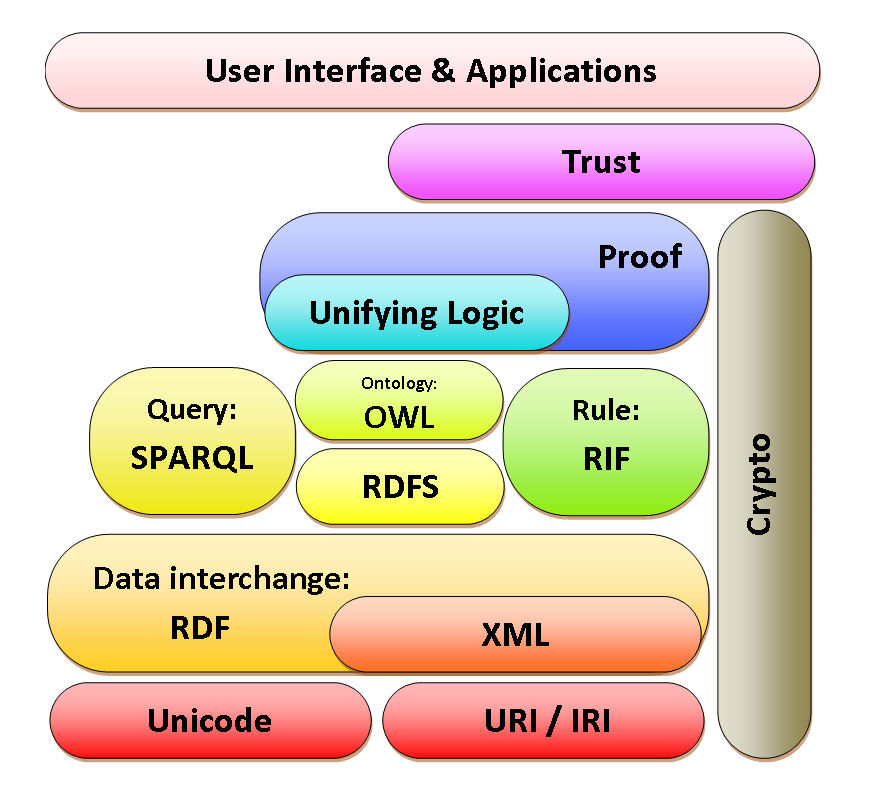
\includegraphics[scale=0.5]{semweb-layers.png}\newline
				\textbf{Figura 1.} Rappresentazione a livelli del Web Semantico.
			\end{center}	
I livelli principali\footnote{Tratto da Realizzazione di moduli JAVA per il trattamento del web semantico di Andrea Costazza} sono:
			\begin{itemize}	
				\item URI/IRI\footnote{Uniform Resource Identifier/Internationalized Resource Identifier}: Il livello degli indirizzi dove indicano una risorsa generica come ad esempio un pagina web
				\item Unicode: Standard di codifica dei set di caratteri internazionali. Questo livello permette che tutte le lingue del mondo possono essere utilizzate per qualsiasi pagina web.
				\item XML\footnote{eXtensible Markup Language}: è un linguaggio di markup, simile all'HTML, che è stato progettato per memorizzare e trasportare i dati. Utilizza dei tag che devono rispettare determinate regole e molto spesso fanno uso dei “namespace”, una sorta di vocabolario di termini, a cui si fa riferimento un URI				
				\item RDF\footnote{Resource Description Framework}: è un linguaggio, proposto dal W3C per rappresentare informazioni sulle risorse in una forma grafica. In questo linguaggio le informazioni sono
esprimibili con asserzioni (statement) costituite da triple formate da
soggetto, predicato e oggetto (identificati come subject, predicate e
object, rispettivamente)\newpage
				\item RDFS\footnote{RDF Schema}: Estensione del RDF, fornisce elementi di base per la descrizione di ontologie, chiamati vocabolari per le risorse RDF. Queste risorse possono essere salvate in un storage di triple che vengono successivamente elaborati con il linguaggio  SPARQL.
				\item OWL\footnote{Ontology Web Language}: è un linguaggio che deriva dalle logiche descrittive, e offre più costrutti rispetto a RDFS. OWL si suddivide in tre categorie: OWL Lite per tassonomie e vincoli semplici, OWL DL per il pieno supporto della logica descrittiva e OWL Full per la massima espressività e la libertà sintattica di RDF. 
				\item SPARQL: è un linguaggio di interrogazione per tipologie di dati rappresentati in RDF; è uno degli elementi cardini per sviluppare il web semantico e consente di estrarre informazioni dalle basi di conoscenza distribuite sul web.
				\item Livello Logiche Descrittive DL: fornisce un formalismo logico per il Semantic Web, le DL si differenziano tra loro per i costruttori ammessi sia sui concetti che sui ruoli.				
			\end{itemize}\newpage			 			
			\item {Resource Description Framework (RDF)}			\newline
			Il \textbf{Resource Description Framework (RDF)}, proposto da W3C, è lo strumento base per la realizzazione del Semantic Web. Esso esprime informazioni sulle risorse che possono essere di qualunque tipo, come ad esempio persone o cose.\newline
I dati espressi possono anche essere, ad esempio, informazioni sulle pagine web, contenuti per i motori di ricerca oppure biblioteche elettroniche, sia aziendali che comunali, contenenti moltissime informazioni.
Per descrivere queste informazioni RDF utilizza:
			\begin{itemize}
				\item Risorse: come già descritto può essere una qualsiasi cosa
				\item Proprietà: è una relazione utilizzata per descrivere una risorsa.
				\item Valore: è il valore assunto dalla proprietà; può essere anche una risorsa.
			\end{itemize}

Le combinazioni tra Risorse, Proprietà e Valori prendono il nome di \textbf{Asserzioni} (statement), cioè una tripla composta da un soggetto (risorsa), un predicato (proprietà) e un oggetto (valore). 
			\begin{center}
				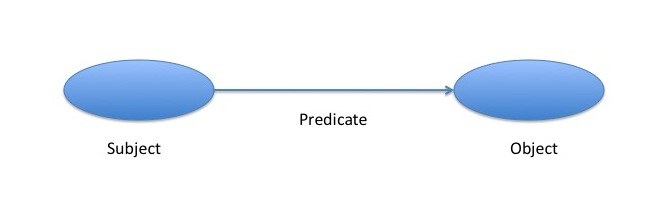
\includegraphics[scale=0.5]{Assertion.jpg}\newline
				\textbf{Figura 2.} Relazione degli statement.
			\end{center}
			
Il soggetto e l'oggetto rappresentano le due risorse, mentre il predicato rappresenta la natura del loro rapporto.
Ecco un esempio di triple in RDF:

<Napoleone> <è nato> <ad Ajaccio>\newline
<Napoleone> <perse> <a Waterloo>.\newline
<Jacques-Louis David> <dipinse l'incoronazione> <di Napoleone>.

Come si evince dall'esempio Napoleone e soggetto di 2 asserzioni e oggetto dell'altra; questa caratteristica importante, cioè quella di avere la stessa risorsa sia in posizione di soggetto e sia in posizione di oggetto, permette di trovare connessioni tra triple e quindi reperire più informazioni.
Si realizza in questo un grafo dove il soggetto e l'oggetto rappresentano i nodi mentre il predicato corrisponde l'arco.

			\begin{center}
				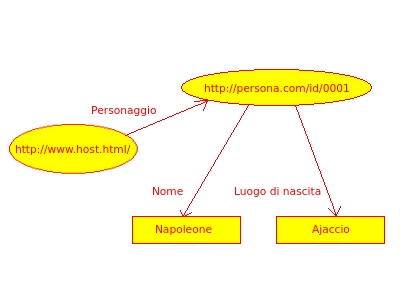
\includegraphics[scale=1]{Napoleone.jpeg}\newline
				\textbf{Figura 3.} Esempio di Grafo.
			\end{center}

che si traduce nel linguaggio rdf:
\begin{lstlisting}[language=XML, basicstyle=\large]
<rdf:Description rdf:about="http://www.host.html/">
	<s:Personaggio rdf:resource="http://persona.com/id/0001"/>
</rdf:Description>
<rdf:Description rdf:about="http://persona.com/id/0001">
 	<s:Nome>Napoleone</s:Nome>
 	<s:Luogo di Nascita>Ajaccio</s:Luogo di Nascita>
</rdf:Description>

\end{lstlisting}

Le risorse, i predicati e i valori però possono assumere qualsiasi forma, le principali forme assunte sono:
			\begin{itemize}
				\item \textbf{URI/IRI}: come ad esempio la risorsa Napoleone può essere contenuta, per esempio, su DBpedia\footnote{ sito internet che offre un progetto aperto e collaborativo per l’estrazione e il riutilizzo di informazioni semi-strutturate dalla Wikipedia in italiano. Fonte http://it.dbpedia.org/}
				\item \textbf{Literals}: sono dei valori costanti, come ad esempio date, numeri o anche stringhe.
			\end{itemize}

Un' altra caratteristica importante del modello RDF e che è le risorse possono essere raggruppate per formare un insieme; tale insieme prende il nome di \textbf{Contenitore} e in RDF può essere di tre tipi:
			\begin{itemize}
				\item \textbf{Bag}, è una lista non ordinata di Risorse e Literals.
				\item \textbf{Sequence}, a differenza di Bag, l'insieme è ordinato.
				\item \textbf{Alternative}, è una lista di risorse che definiscono un'alternativa per il valore singolo di una proprietà\footnote{Fonte Wikipedia.}
			\end{itemize}\newpage		
Per rappresentare semanticamente il modello RDF, si ha bisogno di una estensione chiamata \textbf{RDF Schema}, che fornisce meccanismi per gruppi di risorse correlate e descrive le risorse con le classi, proprietà e valori. Il sistema di classi e delle proprietà di RDF Schema è simile al linguaggio Java e fornisce elementi di base per la descrizione delle ontologie, per vincolare domini e codomini delle relazioni, definire classi di oggetti e relazioni tra classi.
Nelle seguenti tabelle viene descritto le classi e le proprietà utilizzate dal RDF Schema:	\newline
		
		\begin{table}[htb]
		\begin{center}				
		\begin{tabular}{|>{\small}l|>{\small}l|}
				\hline
				\textbf{Nome Classe} & \textbf{Commento}\\				
				\hline
				rdfs:Resource & The class of literal values, e.g. textual strings and integers.\\
				\hline
rdfs:Literal & 	The class of language-tagged string literal values.\\
				\hline
rdf:langString & La classe  language-tagged string literal values.\\
				\hline
rdf:HTML &	The class of HTML literal values.\\
				\hline
rdf:XMLLiteral	& The class of XML literal values.\\
				\hline
rdfs:Class & The class of classes.\\
				\hline
rdf:Property & The class of RDF properties.\\
				\hline
rdfs:Datatype &	The class of RDF datatypes.\\
				\hline
rdf:Statement & The class of RDF statements.\\
				\hline
rdf:Bag	& The class of unordered containers.\\
				\hline
rdf:Seq	& The class of ordered containers.\\
				\hline
rdf:Alt	& The class of containers of alternatives.\\
				\hline
rdfs:Container & The class of RDF containers.\\
				\hline
rdfs:ContainerMembershipProperty & The class of container membership properties.\\
				\hline
rdf:List &	The class of RDF Lists.\\
				\hline
			
		\end{tabular}	
		\caption{Tabella delle classi dell'RDF Schema.}	
		\end{center}	
		\end{table}
		
		\begin{table}[htb]
		\begin{center}			
		\begin{tabular}{|>{\small}l|>{\small}l|>{\small}l|>{\small}l|}
				\hline
			\textbf{Property name} & \textbf{comment}	& \textbf{domain} & \textbf{range}\\
				\hline
rdf:type & The subject is an instance of a class. & rdfs:Resource &	rdfs:Class\\
				\hline
rdfs:subClassOf	& The subject is a subclass of a class. & rdfs:Class &	rdfs:Class\\
				\hline
rdfs:subPropertyOf	& The subject is a subproperty of a property.&	rdf:Property & rdf:Property\\
				\hline
rdfs:domain & A domain of the subject property.& rdf:Property &	rdfs:Class\\
				\hline
rdfs:range & A range of the subject property.&	rdf:Property&rdfs:Class\\
				\hline
rdfs:label & A human-readable name for the subject. &	rdfs:Resource &	rdfs:Literal\\
				\hline
rdfs:comment& A description of the subject resource.& rdfs:Resource &	rdfs:Literal\\
				\hline
rdfs:member & A member of the subject resource. &	rdfs:Resource &	rdfs:Resource\\
				\hline
rdf:first & The first item in the subject RDF list. & rdf:List&	rdfs:Resource\\
				\hline
rdf:rest & The rest of the subject RDF list after the first item. & rdf:List & rdf:List\\
				\hline
rdfs:seeAlso & Further information about the subject resource. & rdfs:Resource & rdfs:Resource\\
				\hline
rdfs:isDefinedBy & The definition of the subject resource.	& rdfs:Resource & rdfs:Resource\\
				\hline
rdf:value &	Idiomatic property used for structured values.&	rdfs:Resource &	rdfs:Resource.\\
				\hline
rdf:subject	& The subject of the subject RDF statement. &	rdf:Statement &	rdfs:Resource\\
				\hline
rdf:predicate &	The predicate of the subject RDF statement. &	rdf:Statement &	rdfs:Resource\\
				\hline
rdf:object & The object of the subject RDF statement.&	rdf:Statement &	rdfs:Resource\\
				\hline		
		\end{tabular}
		\caption{Tabella delle proprietà dell'RDF Schema.}	
		\end{center}	
		\end{table}
		
		\newpage
		\item {Logiche descrittive}\newline
La logica descrittiva\footnote{Description Logics} è una notazione formale utilizzata nella rappresentazione della conoscenza. Ogni nodo, oggetto o categoria, è caratterizzato da un elenco di proprietà.
Dato un particolare dominio di conoscenza, la logica descrittiva individua i concetti primari, le categorie più rilevanti, e successivamente analizza le proprietà degli oggetti, al fine di migliorare la descrizione delle classificazioni e delle sotto-classificazioni del dominio di conoscenza. 

Ogni DL è basata da blocchi sintattici di base che sono:
\begin{itemize}
\item \textbf{Concetti}: corrispondenti a predicati unari che con i quali, combinati tra loro, danno origine a predicati complessi 
\item \textbf{Ruoli}: corrispondenti a predicati binari ed eventualmente operatori
\item \textbf{Individui}: costanti usati solo nelle asserzioni.
\end{itemize}


Una base di conoscenza per le DL è costituito da:
\begin{itemize}
\item un insieme finito di assiomi \textbf{Tbox}(terminalogical box) 
\item un insieme finito di asserzioni \textbf{Abox} (assertional box).
\end{itemize}

Il TBox contiene frasi che descrivono gerarchie di concetti o di ruoli, mentre l'Abox è un insieme finito di asserzioni di concetto o di ruolo (ad esempio, le relazioni tra gli individui e concetti).
Introduciamo adesso un concetto sintattico molto importante per lo sviluppo delle logiche descrittive, cioè il \textbf{linguaggio descrittivo}.
Un linguaggio descrittivo è il linguaggio attraverso cui si esprimono prescrizioni, aventi la funzione di indirizzare il comportamento degli individui.

\textbf{Definizione}. \newline Un linguaggio descrittivo consiste di una terna di insiemi finiti. \textbf{(C, R, Ob)}. Gli elementi di \textbf{C} sono indicati con le lettere A, B, . . . e sono chiamati concetti atomici; gli elementi di \textbf{R} sono indicati con le lettere R, S, . . . e sono detti
ruoli, mentre gli elementi di \textbf{Ob} sono indicati con le lettere a, b, . . . e sono detti nomi degli oggetti\footnote{ http://homes.di.unimi.it/~ghilardi/logica2/DL.pdf) Introduzione alle Logiche Descrittive di Silvio Ghilardi}\newline
Fra i costruttori di concetti annoveriamo certamente gli operatori booleani che indichiamo con $\neg$(negazione), $\sqcap$(intersezione), $\sqcup$(unione). Ci riserveremo anche di usare rispettivamente per il concetto universale $\top$(sempre soddisfatto) e  per il concetto contraddittorio $\bot$(mai soddisfatto).\newline
Un linguaggio descrittivo si può scrivere nel seguente modo $\I = (\Delta^\I,\cdot^\I)$

dove $\Delta^\I$ rappresenta il dominio dell'interpretazione, 
mentre $\cdot^\I$ rappresenta la funzione di interpretazione, che assegna:
\begin{itemize}
\item ad ogni concetto atomico A$\in$\textbf{C} un insieme  $A^{\I}\subseteq \Delta^\I$,\newline
\item ad ogni ruolo R$\in$\textbf{R} R una relazione binaria $R^{\I}\subseteq \Delta^{\I}$ x $\Delta^{\I} $,\newline
\item ad ogni nome di oggetto a$\in$\textbf{Ob} un elemento $a^{\I}\in \Delta^\I$.
\end{itemize} 
Una volta fatta la premessa sul linguaggio descrittivo, definiamo adesso la logica descrittiva di base chiamata $\alc$\footnote{Attribute Language with Complement} e definiamo i seguenti concetti:
\begin{itemize}
\item $\top^{\I}=\Delta^\I$
\item $\bot^{\I}=0$
\item $(C \sqcup  D)^{\I}=C^{\I} \cup D^{\I} $
\item $(C \sqcap  D)^{\I}=C^{\I} \cap D^{\I} $
\item $(\neg C)^{\I}=\Delta^{\I} \setminus C^{\I} $
\item $(\forall R.C)^{\I}=\{a \in \Delta^{I} | (\forall[a,b] \in R^{\I}) (b \in C^{I})\}$
\item $(\exists R.C)^{\I}=\{a \in \Delta^{I} | (\exists[a,b] \in R^{\I})\wedge (b \in C^{I})\}$
\end{itemize}
La logica descrittiva $\alc$ si può estendere per creare logiche più complesse e articolate; tra i vari costrutti importanti abbiamo:\newline
$\N$: si introducono i costruttori $\geq nR$, $\leq nR$, detti restrizioni numeriche, dove n$\in$N, che sono interpretati come segue:\newline
\begin{center}
		$(\geq nR)^{\I}=\{a \in \Delta^{I}|\#\{b \in \Delta^{I} |[a,b] \in R^{\I}\}\geq n\}$\newline$(\leq nR)^{\I}=\{a \in \Delta^{I}|\#\{b \in \Delta^{I} |[a,b] \in R^{\I}\}\leq n\}$\newline
\end{center}

dove $\#\{...\}$ si indica la cardinalità dell'insieme $\{...\}$\newline 
$\Q$: si introducono i costruttori$\geq nR.C$, $\leq nR.C$, detti restrizioni qualificate\newline
\begin{center}
		$(\geq nR.C)^{\I}=\{a \in \Delta^{I}|\#\{b \in C^{I} |[a,b] \in R^{\I}\}\geq n\}$\newline$(\leq nR.C)^{\I}=\{a \in \Delta^{I}|\#\{b \in C^{I} |[a,b] \in R^{\I}\}\leq n\}$\newline
\end{center}
$\Onom$: si introducono gli insiemi finiti di elementi detti nominals ($\{a\} o \{a_1,...a_n\} $) interpretati come segue:
\begin{center}
$\{a\}^{\I}=\{a^{\I}\}$
\end{center}
\begin{center}
$\{a_1,...a_n\}^{\I}=\{a_1^{\I},...a_n^{I}\}$
\end{center}\newpage
Per estendere il linguaggio si dice che $\I$ è modello $\models$ di:\newline
\textbf{TBox} se:
\begin{center}
	$\I \models C \sqsubseteq D$ se e soltanto se $C^{\I} \subseteq D^{\I}$	
\end{center}
\begin{center}
	$\I \models \T$ se e soltanto se $\I \models \Phi \forall \Phi \in \T $
\end{center}

\textbf{ABox} se 
\begin{center}
	$\I \models a:C$ se e soltanto se $ a^{\I} \in C^{\I}$
\end{center} 
\begin{center}
	$\I \models (a,b):R$ se e soltanto se $ (a^{\I},b^{\I}) \in R^{\I}$
\end{center}
\begin{center}
	$\I \models \A$ se e soltanto se $\I \models \phi \forall \phi \in \A $
\end{center}
Infine si definisce \textbf{Base di Conoscenza} $\K$ la coppia ordinata $(\A,\T) $ e l'interpretazione $\I$ è modello della base di conoscenza se:
\begin{center}
	$\I \models \K$ se e soltanto se $\I \models \T$ e $\I \models \A $
\end{center}
\end{enumerate}
		\newpage
	\item \LARGE{\textbf{Mappe on-line per siti web}}
		\begin{enumerate}[label*=\arabic*.]
			\Large
			\item {Introduzione}\newline
La realizzazione del portale è stata resa possibile grazie alle librerie fornite dal sito web Leaflet, accessibile digitando l'indirizzo url http://leafletjs.com/.
			Leaflet è una moderna libreria open-source realizzata in JavaScript e ha lo scopo di rendere interattive le mappe per utilizzarle in qualsiasi piattaforma si voglia, che sia desktop o mobile. Lo sviluppatore di tale libreria è Vladimir Agafonkin che, con l'aiuto di un team di collaboratori dedicati, ha realizzato una semplice e versatile libreria con soli circa 33 KB di memoria, inoltre utilizzando la tecnologia \textbf{HTML5} e \textbf{CSS3} è accessibile sui browser moderni quali Chrome, Firefox, Safari e Internet Explorer. Può essere anche accessibile per i borwser più datati e ha anche una buona e facile documentazione on-line, infine ha un'estesa e vasta gamma di plugin, che si possono facilmente integrare rendendo il più compatto possibile e di facile intuizione.	
			\medskip
			\item Collegamento con la libreria\newline
Per preparare il sito web con la mappa interattiva occorre realizzare le seguenti principali procedure:
			\begin{itemize}
				\item Inserire nel codice HTML nella sezione \textbf{head} il riferimento al file \textbf{"`leaflet.css"`}
				\item Includere il file scritto in JavaScript \textbf{"`leaflet.js"'}
				\item Inserire un elemento div che ha come parametro \textbf{"`id=map"'} nella sezione \textbf{body}
				\item Settare attraverso la tecnologia CSS3 le caratteristiche della mappa attraverso l'id "`map"'.				
			\end{itemize}
Come mostrato nel seguente esempio:
\begin{lstlisting}[language=HTML, basicstyle=\small]
<head>
	<meta charset=utf-8 />
	<title>MAPPA</title>
	<link rel="stylesheet" href="./css/leaflet.css"/>
	<link rel="stylesheet" href="./css/menu.css"/>		
	<script src="./js/leaflet.js"></script>
	<script src="./js/client.js"></script>		
</head>
<body>		
	<div id='map'>
	<div id="loading"><p class="loading">Loading...<p></div>
	</div>					
	<div id="navigation"></div>		
	<script type="text/javascript">
		launch();
	</script>
</body>
\end{lstlisting}\newpage

Il secondo passaggio è quello di creare una mappa interattiva, per farlo occorre collegarsi al sito \textbf{www.mapbox.com}, che fornisce un portale gratuito per creare o modificare una mappa secondo le caratteristiche che si vogliono.\newline
Per fare questo occorre registrarsi al sito web fornendo:
			\smallskip
			\begin{itemize}
				\item Username
				\item Cognome
				\item Nome
				\item Email
				\item Password
			\end{itemize}
			\smallskip
			\medskip
Una volta effettuato l'accesso bisogna cliccare sul pulsante \textbf{New Map Box Editor Project}, in questo modo creerà una nuova mappa da poter modellare a seconda delle proprie necessità.\newline
Una volta creata la mappa, cliccare sul pannello Edit, in queto modo si aprirà una nuova pagina.
Sul pannello in alto a sinistra è indicata la consolle per modellare la mappa. Con il pannello \textbf{Style} possiamo scegliere i colori delle strade, dell'acqua, della terra e pianure e dello sfondo.\newline
Sul pannello \textbf{Data}, invece, possiamo decidere se aggiungere marker, poligoni o linee. Di default verrà utilizzato il colore blue.
Infine sull'ultimo pannello, chiamato \textbf{Project} sono indicate tutti i parametri che servono per caricare la mappa sul portale web, come ad esempio il campo Map ID.
Sistemate tutte le modifiche per confermare il progetto della mappa cliccare sul pulsante Save.\newline
In Figura 4 sono mostrate tutti i pannelli con i relativi campi.
			\begin{center}
				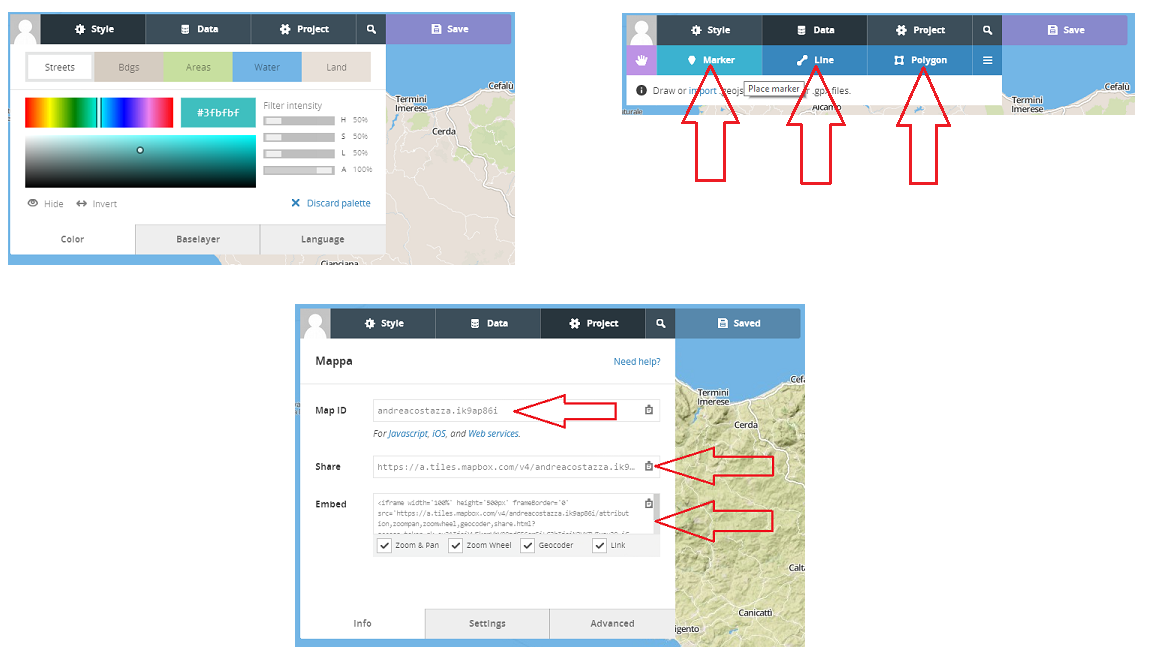
\includegraphics[scale=0.4]{Create_map.png}\newline
				\textbf{Figura 4.} Pannello Consolle.
			\end{center}\newpage			
Per inserire la mappa sul codice sorgente e caricarla nella pagina web, bisogna inizializzarla fornendo le coordinate geografiche della posizione e il livello dello zoom.
Tali informazioni sono reperibile sul sito \textbf{www.mapbox.com} in basso a sinistra come mostrato in Figura 5, e devono essere insirite nella sezione body della file \textbf{index.html}.
			\begin{center}
				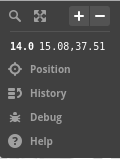
\includegraphics[scale=2.3]{coordinate.png}\newline
				\textbf{Figura 5.} Coordinate e Zoom della Mappa.
			\end{center}
	
Il codice che bisogna inserire si deve mettere nella sezione body ed è il seguente:

\begin{lstlisting}[language=HTML, basicstyle=\large]
<body>		
<div id='map'>
<script type="text/javascript">
	var map=L.map('map')setView([37.583,14.071],9);
</script>
</div>
</body>
\end{lstlisting}
				
Dalla codice si evince che all'interno delle parentesi, sono inserite le coordinate geografiche presenti nella Figura 5, inoltre lo script utilizzato è sempre JavaScript.
Il prossimo passaggio è quello di inserire la mappa utilizzando il comando \textbf{tileLayer}. Tale comando permette di inserire la mappa creata sul sito di Mapbox, definendo lo zoom massimo possibile, gli attributi e l'identificativo della mappa. Di seguito abbiamo il codice sorgente:
\begin{figure}[htb]
\begin{lstlisting}[language=HTML, basicstyle=\large]
<body>		
<div id='map'>
<script type="text/javascript">
var map=L.map('map')setView([37.583,14.071],9);
L.tileLayer('https://{s}.tiles.mapbox.com/v3/{id}/{z}/{x}/{y}.png',{
 maxZoom: 18,
 attribution: 'Map data &copy; 
  <a href="http://openstreetmap.org">OpenStreetMap</a> contributors,'+
  '<a href="http://creativecommons.org/licenses/by-sa/2.0/">CC-BY-SA</a>,'+
	'Imagery c <a href="http://mapbox.com">Mapbox</a>',
	id: 'andreacostazza.ik9ap86i'
	}).addTo(map);
</script>
</div>
</body>
\end{lstlisting}
\end{figure}
\newpage
Sul codice precedente per il caricare la mappa, si nota che nella prima voce è indicato il collegamento ipertestuale della mappa, alla voce \textbf{attribution} sono indicate le licenze, mentre alla voce \textbf{id}, è specificato l'identificativo della nostra mappa, che si ricava dal sito Mapbox alla sezione \textbf{Project} come mostrato in Figura 4 alla voce Map ID.\newline
Seguendo le procedure appena indicate, la mappa verrà visualizzata correttamente nella nostra pagina web.
		\medskip
		\item {Creazione dell'icona}\newline
Attraverso il metodo \textbf{L.Icon} è possibile creare un icona che identifica un determinato punto della mappa. Per prima cosa occorre scegliere un'immagine, dopodiché attraverso \textbf{iconUrl} è possibile caricarla specificando il percorso del file; se si dispone anche di un immagine con l'ombra bisogna caricarla con \textbf{shadowUrl} sempre specificando il percorso del file. Poi bisogna specificare la grandezza dell'icona e dell'ombra, attraverso i parametri \textbf{iconSize} e \textbf{shadowSize} come è evidenziato nel codice seguente. Infine caricare il marker attraverso il metodo \textbf{L.marker}, dove vengono specificate le coordinate.
\begin{figure}[htb]
\begin{lstlisting}[language=HTML, basicstyle=\large]
<body>		
<div id='map'>
<script type="text/javascript">
var map=L.map('map')setView([37.583,14.071],9);
L.tileLayer('https://{s}.tiles.mapbox.com/v3/{id}/{z}/{x}/{y}.png',{
        maxZoom: 18,
        attribution: 'Map data &copy; 
  <a href="http://openstreetmap.org">OpenStreetMap</a> contributors,'+
  '<a href="http://creativecommons.org/licenses/by-sa/2.0/">CC-BY-SA</a>,'+
	'Imagery c <a href="http://mapbox.com">Mapbox</a>',
	id: 'andreacostazza.ik9ap86i'
	}).addTo(map);
var iconBlue= L.icon({
	iconUrl: './icon/marker-icon.png',
	shadowUrl: './icon/marker-shadow.png',
			
	iconSize: [25,41],
	shadowSize: [41,41],
	iconAnchor:[lat,lon],
	shadowAnchor:[lat,lon],
	popupAnchor:[-25,-10]
	});
	
	var marker = L.marker([lat, lon],{icon:iconBlue});		
	marker.addTo(map);
</script>
</div>
</body>
\end{lstlisting}
\end{figure}
		\end{enumerate}
	\newpage
	\item \LARGE{\textbf{SPARQL}}
		\begin{enumerate}[label*=\arabic*.]
			\Large			
			\item {Introduzione}\newline
Il linguaggio \textbf{SPARQL}\footnote{SPARQL Protocol and RDF Query Language} è un linguaggio di interrogazione per dati rappresentati tramite il \textbf{Resource Description Framework (RDF)}.
SPARQL è un elemento essenziale per lo sviluppo del web semantico e consente di estrarre informazioni in tutto il mondo.\newline 
La struttura del database è un insieme di triple "soggetto-predicato-oggetto", però a differenza dell'RDF, le triple possono essere delle variabili, che sono indicate con il punto interrogativo ?, oppure costanti.

\begin{center}	
	\textbf{?title rdf:label ?name}
\end{center}

Nell'esempio proposto il soggetto e l'oggetto sono delle variabili, mentre il predicato è una costante che fa riferimento a rdf\footnote{rdf:http://www.w3.org/TR/rdf-schema/}.\newline
I dati ottenuti, facendo una query\footnote{Interrogazione} allo SPARQL, è una tabella molto simile a quelle utilizzate nei database relazionali in SQL; si tratta di una tabella dove le colonne sono composte dal risultato del soggetto, del predicato e dell'oggetto. 

			\item {Il modello Turtle.}\newline
La sintassi utilizzata nello SPARQL è simile a Turtle\footnote{Terse RDF Triple Language} per esprimere modelli di query. \newline 
Il Turtle è anch'esso un formato per esprimere i dati nel \textbf{Resource Description Framework (RDF)},  anche in questo caso le informazioni vengono rappresentate attraverso le triple, ciascuna delle quali è costituito da un soggetto, un predicato, e un oggetto. Ogni elemento è espresso come indirizzo URI/IRI come mostrato in Figura 6.
			\begin{center}
				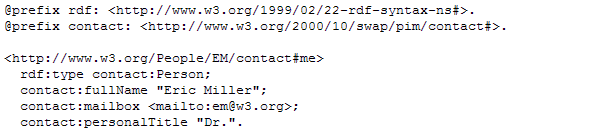
\includegraphics[scale=1]{turtle.png}\newline
				\textbf{Figura 6.} Esempio Codice Turtle.
			\end{center}
Gli indirizzi URI vengono racchiusi tra "<" ed ">" e possono essere abbreviati attraverso il comando \textbf{@prefix}, a cui viene associato un nome che può essere richiamato in diversi parti del file.
Turtle è un'alternativa a RDF/XML, ma a differenza di quest'ultimo, Turtle non si basa su XML ed è più facile da modificare, inoltre risulta molto più leggibile.\newline
Nel 2011, il World Wide Web Consortium (W3C) ha iniziato a lavorare su una versione aggiornata di RDF, ed ha pubblicato la documentazione il 25 febbraio 2014\footnote{La pubblicazione si trova al sito https://www.w3.org/TR/turtle/}.
			\item {Comandi principali}\newline
Il linguaggio SPARQL è composto da tre comandi principali:
	\begin{itemize}
		\item \textbf{PREFIX:} dichiara prefissi e namespace e, come nel Turtle, per
abbreviare il percorso URI si associa un nome che verrà
richiamato all'interno di WHERE (ad es gr:offers può essere
scritto anche <http://purl.org/goodrelations/v1offers>)
		\item \textbf{SELECT:} identifica le variabili che verranno visualizzate, sotto forma di tabella, dal risultato dell' interrogazione. È spesso
accompagnato da *, che seleziona tutte le variabili di una
interrogazione, e DISTINCT, che esclude dal risultato i valori
duplicati;
		\item \textbf{WHERE:} seleziona il criterio di selezione da applicare ai dati; è composto da un blocco, delimitato dalle parentesi graffe (\{...\}),
dove al suo interno può esserci una o più triple, separati da un
punto fermo.
	\end{itemize}
Come in SQL, anche in SPARQL esiste il comando \textbf{FROM}, contenente un
indirizzo IRI, che identifica tutto il set di dati presenti, dove l'interrogazione dovrà essere svolta; è spesso accompagnato dal comando NAMED usato per specificare più indirizzi IRI.
Inoltre SPARQL fornisce diversi comandi per una maggiore flessibilità sulle
interrogazioni. Nella tabella seguente sono riportate quelle più utilizzate:
\begin{table}[htb]
		\begin{center}				
		\begin{tabular}{|>{\small}l|>{\small}l|>{\small}l|}
				\hline
				\textbf{Nome Comando} & \textbf{Cosa fa} & \textbf{Attributi}\\				
				\hline
FILTER: & Filtra i valori visualizzati. & \textbf{regex} si utilizza per espressioni regolari.\\
				\hline
OPTIONAL: & Prevede l'assenza di alcuni termini & Le variabili compariranno prive di valore.\\
				\hline
ORDER BY: & Ordina il risultato in base ad una variabile specifica. & DESC ordinamento decrescente. \\
				\hline
LIMIT: & Limita la visualizzazione. & Accompagnata da valori numerici \\
				\hline
a:	& Visualizza le classi a cui appartiene una variabile. & Alternativa a rdf:type\\

				\hline			
		\end{tabular}	
		\caption{Tabella dei comandi principali di SPARQL.}	
		\end{center}	
\end{table}\newpage
			\item {Libreria javascript per interrogazioni SPARQL}\newline
			Per fare un interrogazione in SPARQL JavaScript ha bisogno di una chiamata AJAX\footnote{Vedi Capitolo 4 paragrafo 4} e della codifica JSON\footnote{Vedi Capitolo 4 paragrafo 3}.
Nel progetto sono date rispettivamente dalla variabile \textbf{xmlhttp}, che fa la chiamata AJAX tramite il metodo \textbf{getHTTPObject()} e restituisce il risultato tramite \textbf{responseText}.
La richiesta AJAX, inoltre, utilizza \newline \textbf{setRequestHeader("Accept", "application/sparql-results+json");} \newline in questo modo i risultati ottenuti sono visualizzati secondo la codifica JSON.
Il codice utilizzato nel progetto è il seguente:
			\begin{figure}[htb]
\begin{lstlisting}[language=HTML, basicstyle=\large]
<body>		
<div id='map'>
<script type="text/javascript">
//Created SPARQL query
function createSparqlQuery(endpoint,query,map,callback){	
 var querypart = "query=" + escape(query);
 // Get our HTTP request object.
 var xmlhttp = getHTTPObject(); //Called AJAX
 //Include POST OR GET
 xmlhttp.open('POST', endpoint, true); 
 xmlhttp.setRequestHeader('Content-type',
 	'application/x-www-form-urlencoded');
 xmlhttp.setRequestHeader("Accept", "application/sparql-results+json");	
 xmlhttp.onreadystatechange = function() {
  if(xmlhttp.readyState==4 ){
   if(xmlhttp.status==200){				
	 callback(xmlhttp.responseText,map); //JSON code
	 }else
	// Error
	alert("Error: Status: "+ xmlhttp.status + "Response: "
	+ xmlhttp.responseText);
	}	
 };
 // Send the query to the endpoint.
 xmlhttp.send(querypart);	
}
</script>
</div>
</body>
\end{lstlisting}
\end{figure}\newline
Basta scrivere la query utilizzando la nomenclatura dello SPARQL descritta precedentemente e fornire l'indirizzo URI della base di conoscenza; la variabile utilizzata nel progetto per scrivere la query è \textbf{query}, mentre per far riferimento alla base di conoscenza si utilizza endpoint.\newpage
		\end{enumerate}
		\item \LARGE{\textbf{Ontologie per la rappresentazione dei servizi pubblici}}
		\begin{enumerate}[label*=\arabic*.]
			\Large
			\item Menù gerarchici.
			\item Linked Open Data per i servizi pubblici
			\item Codifica JSON.
			\item Chiamata AJAX.
		\end{enumerate}
\end{enumerate}
\end{document}
